% \section{GPU-Native JHQ}
% \label{sec:method1}
% \subsection{Execution and representation}
% The transform, codebooks and hierarchy follow JHQ. Batched matrix
% multiplication applies the orthogonal transform; IVF routing selects lists,
% lookup tables score primary codes, and survivors access residual codes.

% Warp lanes score different candidates at the same subspace $m$. A scan copy in
% subspace-major $[M,N]$ order makes their byte reads adjacent, providing standard
% coalescing. Packing four byte codes into a 32-bit word reduces loads, address
% calculations and loop iterations; registers handle unpacking. The logical code
% volume is unchanged.

% \subsection{Cartesian-factorised primary distance tables}
% \label{sec:designspace}
% For subspace $m$, $T_m[c]=\lVert q'_m-C_m[c]\rVert_2^2$. The Cartesian
% codeword construction partitions the coordinate sum exactly:
% \begin{equation}
% T_m[c]=T_m^{\mathrm{hi}}[c\gg4]+T_m^{\mathrm{lo}}[c\bmod16].
% \label{eq:split}
% \end{equation}
% Two 16-entry tables replace 256 entries. Construction evaluates
% $32(D_s/2)$ coordinate contributions instead of $256D_s$, reducing this
% arithmetic by $16\times$ and table entries by $8\times$. These counts do not
% predict search speedup. Exactness holds in real arithmetic; floating-point
% association and tie order can differ. Equal $G$-way grouping stores
% $G2^{8/G}$ entries and requires $G$ lookups per candidate--subspace.

% The scan admits a table into shared memory when
% \begin{equation}
% 40\,\texttt{BLOCK}+4MG2^{8/G}\le\texttt{smem\_optin},
% \label{eq:resid}
% \end{equation}
% where the first term is candidate scratch. On the tested device,
% $\texttt{smem\_optin}=101{,}376$ bytes leaves $94$--$59$\,KiB as
% \texttt{BLOCK} rises from 128 to 1024. At $M=96/384$, full tables need
% $96$/$384$\,KiB and use the global-memory path; split tables need
% $12$/$48$\,KiB and fit throughout this range (Figure~\ref{fig:lut}). Global loads may hit cache;
% Section~\ref{sec:rq3} measures the performance trade-off.
% \begin{figure}[tbp]
% \centering
% 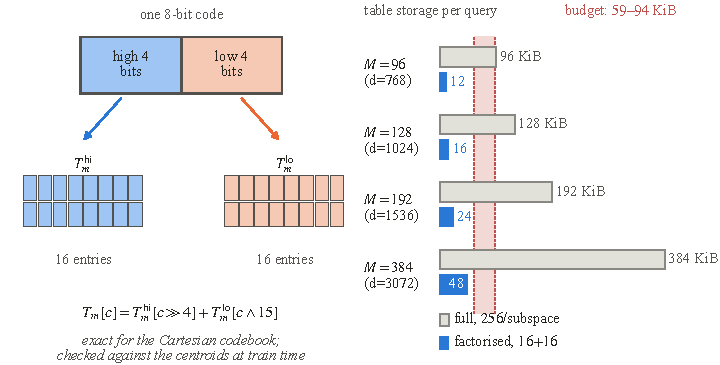
\includegraphics[width=\linewidth]{figs/fig_lut.pdf}
% \caption{Cartesian factorisation and table storage. The band shows shared
% memory available after candidate scratch, not measured cache behaviour.}
% \label{fig:lut}
% \end{figure}

% \subsection{Selective refinement and the policy question}
% Only $c_k$ survivors are scored using primary reconstruction plus residual.
% Accessing residuals during the broad scan would increase this work from
% $O(c_kd)$ towards $O(n_cd)$. The remaining decision is $c_k=\alpha k$:
% \emph{how many primary survivors should be refined}?




\section{GPU Execution for JHQ}
\label{sec:gpu_execution}
We accelerate primary screening through candidate-parallel access and exact table factorization, preserving JHQ's transform, codebooks, and hierarchy.

\subsection{Candidate-Parallel Scanning}
\label{sec:candidate_parallel}
Warp lanes score different candidates at the same subspace. A subspace-major scan copy, $[M,N]$, places consecutive candidates' codes contiguously for coalesced access. Packing four byte codes into a 32-bit word reduces loads, address calculations, and loop iterations, with register-based unpacking. These optimizations preserve logical code volume but leave $256M$ query-specific distance entries, potentially exceeding shared-memory capacity.

\subsection{Exact Distance-Table Factorization}
\label{sec:table_factorization}
For $B=D_s=8$, JHQ's Cartesian codebook associates the high and low four bits with separate coordinate groups. Squared-distance additivity gives
$
T_m[c]=T_m^{\mathrm{hi}}[\lfloor c/16\rfloor]+T_m^{\mathrm{lo}}[c\bmod16],
\label{eq:table_factorization}
$
where each subtable stores distances to 16 group codewords. This reduces storage eightfold and construction arithmetic from $256D_s$ to $32(D_s/2)$ coordinate contributions, a $16\times$ reduction relative to independent full-table construction. Exactness holds in real arithmetic; floating-point association and ties may differ. Arbitrary learned PQ subcodebooks do not generally provide this separability.

\subsection{Grouping and Refinement Trade-offs}
\label{sec:grouping_tradeoff}
Equal $G$-way grouping, $G\in\{1,2,4,8\}$, requires $G2^{8/G}$ entries per subspace and $G$ lookups per candidate--subspace pair. Both $G=4$ and $G=8$ store 16 entries but require different lookup work; smaller tables therefore need not produce faster scans.

Tables use shared memory when
$
40\cdot\mathrm{BLOCK}+4MG2^{8/G}\leq S_{\mathrm{opt}},
\label{eq:shared_memory_budget}
$
where the first term is candidate scratch, table entries occupy four bytes, and $S_{\mathrm{opt}}$ is the configured per-block limit. Otherwise, tables use global memory. With $S_{\mathrm{opt}}=101{,}376$ bytes and block sizes 128--1024, split tables at $M=96/384$ require 12/48~KiB and fit, whereas full tables require 96/384~KiB and do not. Caching and instruction costs still determine the realized benefit.

Only primary survivors access residual codes, preserving $O(n_cM)$ screening and $O(c_kd)$ refinement. Faster screening leaves refinement work unchanged, motivating workload-level budget selection.